 \section{Electromagnetic Calorimeter}
Directly outside of the tracking system lies the electromagnetic calorimeter 
(ECAL) of CMS. The driving criteria of the ECAL design is to provide capability
to detect and measure the decay to two photons of the Higgs Boson. The 
ECAL is designed with the objective of a
fast response time, a fine granularity and resistance to the effects of radiation.
Therefore, recently advanced lead tungstate (PbWO$_{4}$) technology was chosen. 
A preshower detector is placed in front of the endcap. Avalanche photodiodes (APDs)
are used as photodetectors in the barrel and vacuum phototriodes (VPTs) in the
endcaps.
The layout of the CMS ECAL is shown in Figure \ref{fig:ECALLayout}.
The barrel part of the ECAL (EB) covers the pseudorapidity range $|\eta|<1.479$
the endcap part covers the rapidity range $1.479<|\eta|<3.0$.
\begin{figure}[hb]
  \centering
	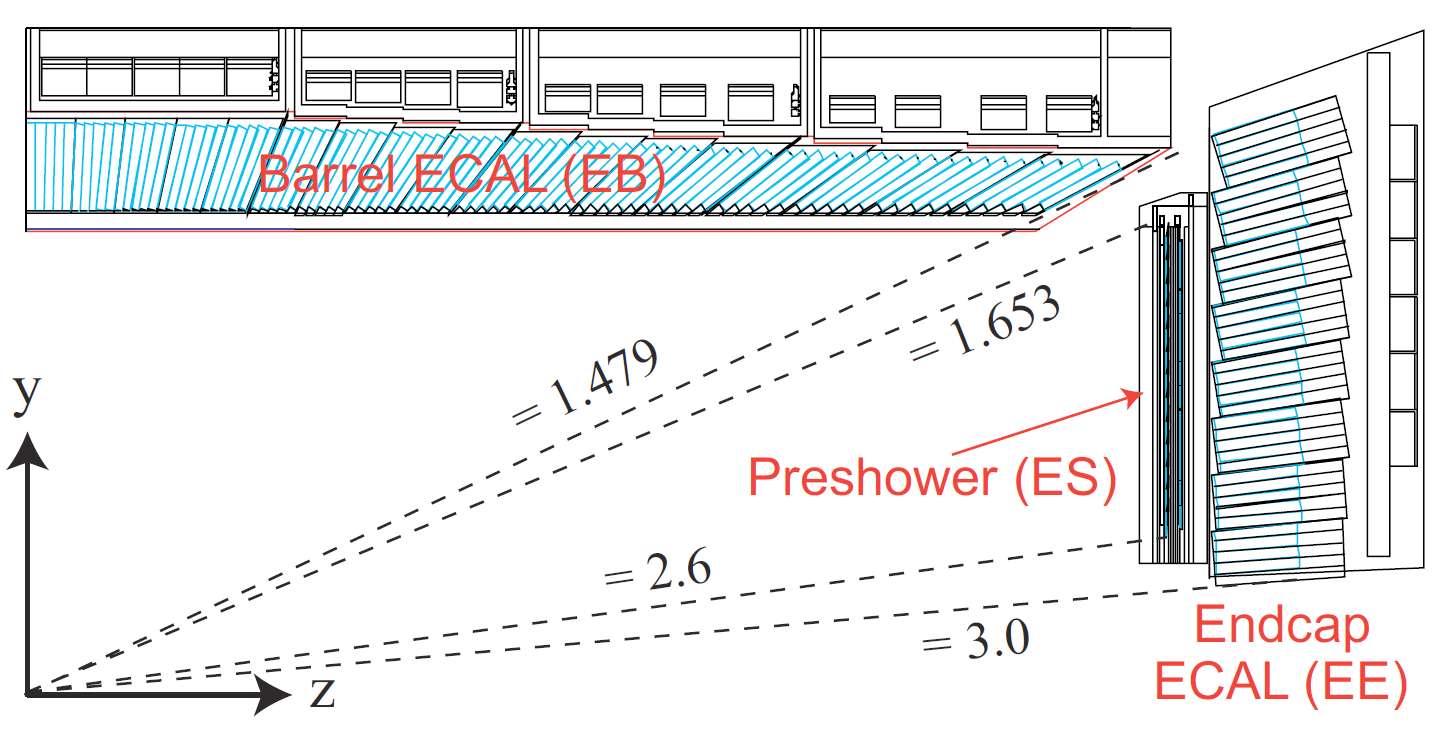
\includegraphics[width=0.75\textwidth]{images/ECALPreshower.png}
  	\caption[ECAL Layout]
   	{CMS Electromagnetic Calorimeter Layout}
	\label{fig:ECALLayout}
\end{figure}
\subsection{Lead Tungstate Crystals}
The ECAL is composed of 75,848 PbWO$_{4}$ crystals: 61,200 mounted in the 
central barrel part, closed by 7,324 crystals in each of the two endcaps. They 
have a high density of 8.28$g/cm^{3}$ and a short radiation length of 0.89cm. 
The Moli$\grave{e}$re radius (radius of a cylinder containing 90\% of the shower's energy deposit) 
is only 2.2cm. These characteristics result in a fine granularity and a compact
calorimeter. Furthermore, the scintillation decay time of these crystals is of the
same order of magnitude as the LHC bunch crossing time whereby 80\% of 
the light is emitted in 25ns. 
\subsection{ECAL Energy Resolution}
The energy resolution in the ECAL can be parameterized as in the following equation:
\begin{displaymath}
\left(\frac{\sigma}{E}\right)^{2}=\left(\frac{S}{\sqrt{E}}\right)^{2}+\left(\frac{N}{E}^{2}\right)+C^{2}
\label{eqn:ECALResolution}
%%%cite equation
\end{displaymath}
where $S$ is the stochastic term, $N$ the noise term, and $C$ the constant term. 
The individual contributions are described in the following paragraphs.

The stochastic term in equation \ref{eqn:ECALResolution} has four primary contributions:
A random event-to-event fluctuation in the lateral containement of the
electromagnetic decay and subsequent photon and electron-positron production,
a photoelectron statistics contribution, fluctuations in the energy
deposited in the preshower absorber and dead material in front of the calorimeter. %%%double check this
This shower containment term is expected to be 1.5\% when energy is 
reconstructed by summing an array of 5 $\times$ 5 crystals and 2\%
when using 3 $\times$ 3 crystals. 
The noise term, N, has three main contributions: electronics noise, digitization 
noise, and pileup noise. The digitization and electronics noise (or Electromagnetic Interference)
is a consequence of any electronic system and creates small amounts of
interference in the output; this interference was measured in the test beam and 
found to be $\approx$ 40 MeV/channel. 
Pileup noise occurs if additional particles from pileup events reach the 
calorimeter causing signals that overlap. 
Finally, the primary contributions to the constant term, C, is non-uniformity
of the longitudinal light collection, intercalibration errors and leakage from the 
back of the crystal. 

In 2004 an electron test beam with momenta between 20 and 250 GeV 
was used to measure the parameters in equation \ref{eqn:ECALResolution}
results by measuring the energy in a 3 $\times$ 3 crystal region. A typical
energy resolution was found to be:
The energy resolution in the ECAL can be parameterized as in the following equation:
\begin{displaymath}
\left(\frac{\sigma}{E}\right)^{2}=\left(\frac{2.8\%}{\sqrt{E}})^{2}\right)+\left(\frac{0.12}{E}^{2}\right)+(0.30\%)^{2}
\label{eqn:ECALResolution}
%%%cite equation
\end{displaymath}
A later test in 2006 showed a 10\% improvement of the noise performance.



